\documentclass[10pt]{article}
\usepackage{graphicx}
\usepackage{algorithm}
\usepackage{algpseudocode}

\begin{document}
\title{CSE616 Neural Networks and Their Applications\\
Project 2 Submission}
\author{Ayman Wagih Mohsen (2000728)}
\maketitle

\setcounter{section}{3}
\section{Main Results}

\subsection{Experimental Results}
Fast R-CNN uses 3 pretrained ImageNet Models:\\
1. The small (S) size CaffeNet, which is based on AlexNet.\\
2. The medium (M) size VGG\_CNN\_M\_1024.\\
3. The large (L) size VGG16.\\
Training and testing are single sale and the length of the shortest image side s=600.

\subsection{VOC 2007, 2010 and 2012 results}
The PASCAL Virtual Object Classes (VOC) project is an object classification competition that had a series of challenges spanning from 2005 till 2012.\\
The mean average precision (mAP) of Fast R-CNN on VOC 2012 was the highest at its time (65.7\%). It was also the fastest contestant on that dataset.\\
Fast R-CNN was surpassed only by SegDeepM on VOC 2010.\\
As for VOC 2007 Fast R-CNN is a large improvement over the other contestants.

\subsection{Training and testing time}

Truncated singular value decomposition (SVD) helps in fully connected (FC) layers. For example if the fc6 layer has weights in the shape of a $25088\times4096$ matrix, then by using SVD we can use the largest 1024 singular values only. Saving test time at the cost of a little precision.

\begin{center}
\begin{table}
\caption{Fast R-CNN train and test time compared to R-CNN}
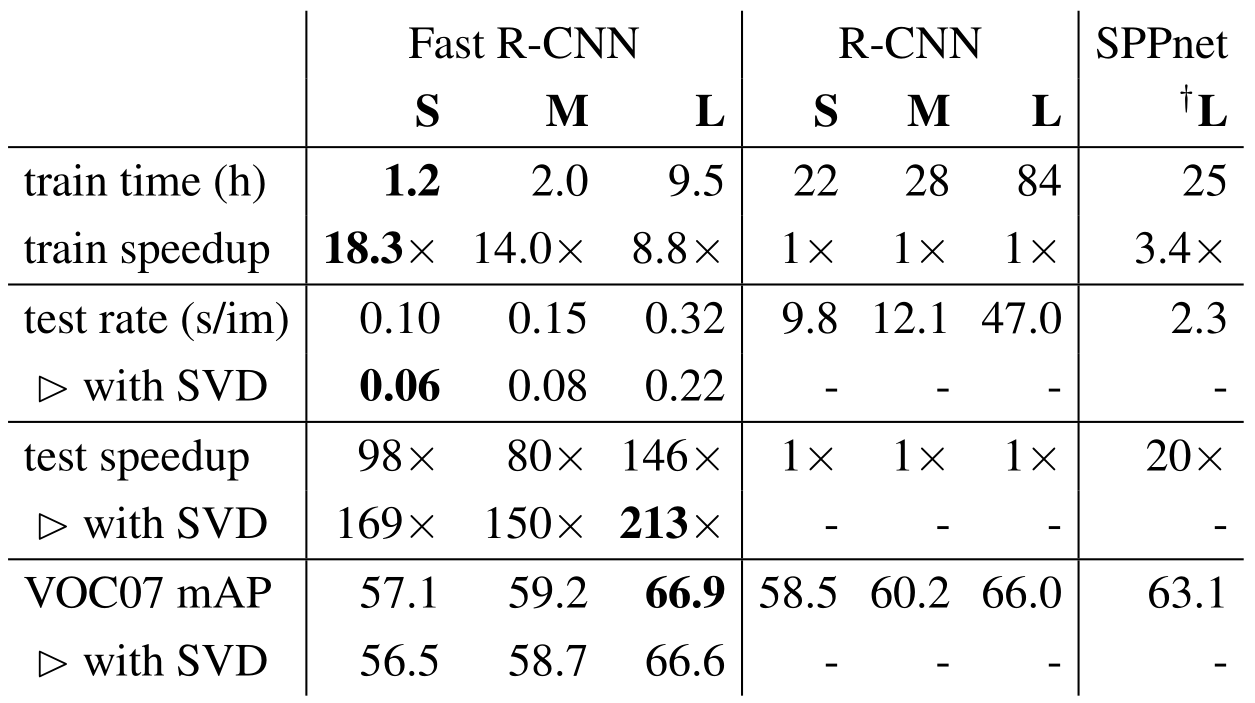
\includegraphics[width=0.9\textwidth]{20220602 1 speed.PNG}
\DeclareGraphicsExtensions{.png}
\end{table}
\end{center}

\subsection{Which layers to fine-tune?}
With very deep networks it is not enough to fine tune just the fully connected layers. In the fast R-CNN study using the large VGG16 net, it was revealed that it is best to fine-tune the last 9 conv layers out of the total 13 ($conv3_1$ and up). And this increased mAP from 61.4\% to 66.9\%. Fine-tuning starting from earlier layers has more impact on train time than on mAP.\\
As for medium and small nets, it was shown that fine-tuning conv layers has too little of an impact on the mAP. So fine-tuning the FC layers only is enough.


\section{Design evaluation}

\subsection{Does multi-task training help?}
Multi-task learning is when a network is trained for multiple tasks simultaneously to save redundant calculations at test time, espacially in the early layers. The loss function becomes a weighted sum of sub-task loss functions. From the fast R-CNN study, it turns out that multi-task training for tasks A and B sometimes helps the network get better at task A than just training for task A. When the network was jointly trained for object classification and bounding box regression, it got better by 0.8 to 1.1 mAP at classification than training just for classification. This positive effect is consistent assuming the tasks are somehow related.

\subsection{Scale invariance: to brute force or finesse?}
Image scale is the length of its shortest side. Brute-force learning here means that all images are in single scale (of s=600). The aspect ration is kept the same. While multi-scale learning uses image pyramids at scales of s={480, 576, 688, 864, 1200}. The fast R-CNN concludes that there is no need to train at multiple scales, as the gain in mAP is negligible compared to the increase in training memory requirements. This applies especially to the deep models like VGG16.

\subsection{Do we need more training data?}
When the number of images in VOC 2007 dataset was tripled to 16500 by augmenting with VOC 2012 dataset, the mAP improved from 66.9\% to only 70.0\%. When the VOC 2010 dataset was augmented with VOC 2007 to 21500 images and the learning rate is lowered by $0.1\times$ each 40k iterations, mAP improved more significantly from 66.1\% to 68.8\%. The same was done with VOC 2012 dataset and mAP improved from 65.7\% to 68.4\%.

\subsection{Do SVMs outperform softmax?}
R-CNN uses softmax, while fast R-CNN was tested with softmax and SVM. Softmax slightly outperforms support vector machines (SVMs) by 0.1 to 0.8 mAP.

\subsection{Are more proposals always better?}
A proposal here means a candidade region of interest (RoI). Object detectors can use a sparse set of object proposals (e.g. selective search) or a dense set (e.g. DPM). For sparse set, as the proposal count increases, mAP rises then falls slightly, peaking around 3000 or 4000 proposals. With densely generated boxes is was concluded that mAP drops with larger proposal count.

\subsection{Preliminary MS COCO results}
The large VGG16 net based fast R-CNN was also trained on Microsoft COCO dataset with 80k images for 240k iterations, giving mAP of 35.9\%.


\section{Conclusion}
An improvement on Region-based CNN (R-CNN) was proposed called Fast R-CNN. The new object detection technique is orders of magnitude faster at training and testing, allowing for more experimentation to study the effects of various hyperparameters on mean average precision (mAP). The speedup was achieved as follows: instead of passing each region of interest (RoI) again and again through the CNN, the CNN is run on the whole image followed by a novel stage called ROIPooling. This eliminates redundant calculations.


\begin{thebibliography}{9}

\bibitem{paper1}
Ross Girshick (ICCV 2015) "Fast R-CNN" https://arxiv.org/abs/1504.08083

\end{thebibliography}

\end{document}



